\documentclass[times, utf8, seminar, numeric]{fer}
\usepackage{booktabs, url, hyperref}
\usepackage{verbatim}
\usepackage{moreverb}
\usepackage{subfigure}
\usepackage{caption}
\usepackage{epstopdf}

\hypersetup{
   colorlinks,
   citecolor=black,
   filecolor=black,
   linkcolor=black,
   urlcolor=black
}

%dodatak za programski kod
\usepackage{listings}
\usepackage{color}
\usepackage{setspace}
\definecolor{dkgreen}{rgb}{0,0.6,0}
\definecolor{gray}{rgb}{0.5,0.5,0.5}
\definecolor{mauve}{rgb}{0.58,0,0.82}

\lstset{frame=tb,
  language=Java,
  aboveskip=3mm,
  belowskip=3mm,
  showstringspaces=false,
  columns=flexible,
  basicstyle={\small\ttfamily},
  numbers=left,
  numberstyle=\small\color{gray},
  keywordstyle=\color{blue},
  commentstyle=\color{dkgreen},
  stringstyle=\color{mauve},
  breaklines=true,
  breakatwhitespace=true,
  tabsize=2
}


\begin{document}

\nocite{saitou}\nocite{phylpro}\nocite{wiki}\nocite{mbt}

% TODO: Navedite naslov rada.
\title{Algoritam "Neighbor joining"}

% TODO: Navedite vaše ime i prezime.
\author{\itshape{Filip Beć}\\
				 \itshape{Zorana Ćurković}\\
				 \itshape{Goran Gašić}\\
				 \itshape{Melita Kokot}\\
				 \itshape{Dino Šantl}\\
				 \itshape{Igor Smolkovič}
				 }

% TODO: Navedite ime i prezime mentora.
\voditelj{\itshape{Dr. sc. Mirjana Domazet-Lošo}\\ \itshape{Doc. dr. sc. Mile Šikić}}

\maketitle

\tableofcontents

\chapter{Opis algoritma}

Algoritam \emph{Neighbor joining} služi za izgradnju filogenetskog stabla. Ulaz algoritma su evolucijske udaljenosti (matrica udaljenosti čvorova). Izlaz algoritma je stablo s težinskim bridovima. Cilj algoritma je izgraditi minimalno razapinjajuće filogenetsko stablo. Algoritam nužno ne pronalazi takvo stablo, ali rješenja su često minimalna razapinjajuća filogenetska stabla ili blizu toga \cite{saitou}. Glavni razlog je smanjenje vremenske složenosti jer u praksi nije izvedivo ispitivanje svih mogućih stabala. Stablo se gradi od dna prema vrhu. Algoritam je pohlepan jer za jednom sparene čvorove ne ispituje točnost tog koraka.

Algoritam se sastoji od dva dijela: uparivanje čvorova i završni korak. Algoritam kreće od matrice udaljenosti nad kojom zaključuje koja dva čvora je potrebno upariti. Kada su poznata dva čvora koja se trebaju upariti, stvara se novi čvor koji se spaja s dva odabrana. Dva odabrana čvora se brišu iz matrice udaljenosti, a novi čvor se doda u matricu udaljenosti. Taj postupak se izvršava $N-3$ puta, gdje je $N$ početni broj čvorova. Završni korak uzima zadnja tri čvora koja su ostala u matrici udaljenosti, stvara novi čvor i spaja novi čvor s tri zadnja čvora u matrici udaljenosti. Formalno algoritam izgleda ovako:
\begin{enumerate}
	\item \textbf{Ulaz}: matrica udaljenosti
	\item Na temelju trenutne matrice udaljenosti izračunaj matricu \textbf{Q}
	\item U matrici \textbf{Q} pronađi najmanju vrijednost $Q(i,j)$ i pripadajuće čvorove $(i,j)$.
	\item Stvori novi čvor $w$ i dva nova brida: $(w,i)$ i $(w,j)$ te izračunaj udaljenosti $d(w,i)$ i $d(w,j)$ i zapiši ih na pripadajući brid.
	\item Iz matrice udaljenosti izbriši čvorove $i$ i $j$, te dodaj u matricu novi čvor $w$ - potrebno je izračunati udaljenosti do novoga čvora $w$
	\item Ako postoji više od tri čvora u matrici udaljenosti skoči na korak 2.
	\item Stvori novi čvor $w$ i napravi tri brida s preostalim čvorovima u matrici udaljenosti te izračunaj i pridruži vrijednost bridovima 
\end{enumerate}

\section{Matrica Q}
Matrica \textbf{Q} pomoćna je matrica iz koje se određuje par čvorova koji će biti susjedni. Matrica \textbf{Q} kao kriterij uzima osim udaljenosti čvorova $i$ i $j$ utjecaj njihovih susjeda. Dokaz da najmanja vrijednost matrice \textbf{Q} pripada susjednim čvorovima dan je u \cite{saitou}. Matrica \textbf{Q} izračunava se na sljedeći način:

\begin{equation}
	Q(i,j) = (r-2) d(i,j) - \sum_{k=1}^{r}d(i,k) - \sum_{k=1}^{r}d(j,k)
\end{equation}
, gdje su $i$, $j$ indeksi čvorova, $r$ je trenutni broj čvorova u matrici udaljenosti. Oznake $d(i,j)$, $d(i,k)$ i $d(j,k)$ predstavljaju vrijednosti u matrici udaljenosti. Čvorovi $i$ i $j$ moraju biti različiti.

\section{Računanje vrijednosti bridova}

Nakon što se stvore novi bridovi u stablu potrebno je odrediti njihovu vrijednost. U svakom koraku uparivanja stvore se dva nova brida. U završnom koraku stvore se tri nova brida.

Nakon što se čvorovi $i$ i $j$ proglase susjednima stvara se novi čvor $w$. Potrebno je odrediti udaljenosti $d(i, w)$ i $d(j,w)$. Udaljenosti se određuju prema formulama:

\begin{equation}
d(i,w) = \frac{1}{2}d(i,j)+\frac{1}{2(r-2)} \left [ \sum_{k=1}^{r}d(i,k) - \sum_{k=1}^{r}d(j,k) \right ]
\end{equation}
, gdje je $r$ trenutni broj čvorova u matrici udaljenosti.

Kako vrijedi $d(i,j)=d(i,w)+d(j,w)$, iz toga slijedi:
\begin{equation}
d(j,w) = d(i,j) - d(i,w)
\end{equation}

\section{Računanje udaljenosti do novog čvora}

Pri dodavanju novog čvora u matricu udaljenosti potrebno je izračunati udaljenost od svih starih čvorova do novog čvora $w$. Udaljenost se računa prema formuli: 

\begin{equation}
d(k,w) = \frac{1}{2} \left [ d(i,k) + d(j,k) - d(i,j) \right ]
\end{equation}
, gdje je $k$ bilo koji stari čvor u matrici udaljenosti. Čvorovi $i$ i $j$ su upravo spojeni čvorovi. 

\section{Složenost algoritma}

Algoritam mora izvršiti korak uparivanja $N-3$ puta, gdje je $N$ broj čvorova u početnoj matrici udaljenosti. U svakom koraku potrebno je izračunati matricu \textbf{Q} koja je dimenzije $r\times r$, gdje je $r$ trenutni broj čvorova. Ako se pretprocesiraju sume u prije navedenim formulama u $O(N^2)$ vremenskoj složenosti, tada se matrica \textbf{Q} može izračunati u $O(N^2)$ vremenskoj složenosti. Zbog toga je ukupna vremenska složenost algoritma $O(N^3)$. Memorijska složenost je $O(N^2)$ jer se pamti matrica udaljenosti.

\chapter{Primjer izvođenja}

Raspolažemo skupom od $5$ taksona $(\textup{Dog},\textup{Cat},\textup{Rabbit},\textup{Monkey},\textup{Cow})$ te pridanim udaljenostima među njima definiranim matricom udaljenosti:
\begin{table}[h]
	\centering
    \begin{tabular}{|l|l|l|l|l|l|}
    \hline
    ~ & Dog  & Cat  & Rabbit  & Duck  & Swan  \\ \hline
    Dog & 0  & 5  & 17 & 15 & 13 \\ \hline
    Cat & 5  & 0  & 9  & 19 & 14 \\ \hline
    Rabbit & 17 & 9  & 0  & 20 & 16 \\ \hline
    Duck & 15 & 19 & 20 & 0  & 12 \\ \hline
    Swan & 13 & 14 & 16 & 12 & 0  \\ \hline
    \end{tabular}
\end{table}

Algoritam će biti proveden u $N-3=2$ koraka. \newline

\begin{figure}[htb]
\centering
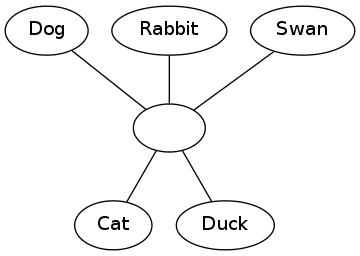
\includegraphics[scale=0.6]{./img/pocetni.png}
\caption{Početno stablo}
\end{figure}

\newpage
\section{Korak 1}
Izračunamo matricu $Q$ te tražimo par $(i,j)$ koji ima najmanju vrijednost:

\begin{table}[h]
	\centering
    \begin{tabular}{|l|l|l|l|l|l|}
    \hline
    ~ & Dog  & Cat  & Rabbit  & Duck  & Swan  \\ \hline
    Dog & 0   & -82 & -61 & -71 & -66 \\ \hline
    Cat & -82 & 0   & -82 & -56 & -60 \\ \hline
    Rabbit & -61 & -82 & 0   & -68 & -69 \\ \hline
    Duck & -71 & -56 & -68 & 0   & \textbf{-85} \\ \hline
    Swan & -66 & -60 & -69 & -85 & 0   \\ \hline
    \end{tabular}
\end{table}

$i = \textup{Duck}, j = \textup{Swan}, Q_{min} = -85$. Taksone Duck i Swan spajamo u novi čvor $\textup{node1}$ te računamo udaljenosti: 

\indent $d(\textup{Duck},\textup{node1}) = 7.833$, \newline
\indent $d(\textup{Swan},\textup{node1}) = 4.166$


Preostale udaljenosti $d(k,\textup{node1})$ definirane su novom matricom udaljenosti :

\begin{table}[h]
	\centering
    \begin{tabular}{|l|l|l|l|l|l|}
    \hline
	~ & Dog  & Cat    & Rabbit  & node1 \\ \hline
    Dog     & 0  & 5    & 17 & 8     \\ \hline
    Cat   & 5  & 0    & 9  & 10.5  \\ \hline
    Rabbit     & 17 & 9    & 0  & 12    \\ \hline
    node1 & 8  & 10.5 & 12 & 0     \\ \hline
    \end{tabular}
\end{table}

\begin{figure}[htb]
\centering
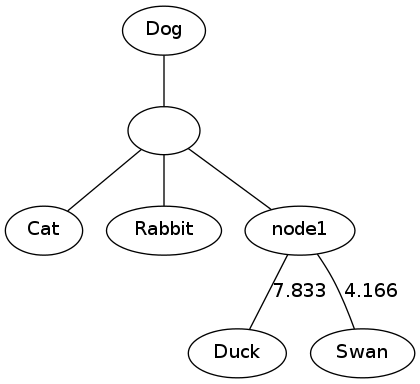
\includegraphics[scale=0.6]{./img/prvi.png}
\caption{Trenutno stablo}
\end{figure}

\newpage
\section{Korak 2}
Izračunamo matricu $Q$ te tražimo par $(i,j)$ koji ima najmanju vrijednost:

\begin{table}[h]
	\centering
    \begin{tabular}{|l|l|l|l|l|l|}
    \hline
~     & Dog     & Cat     & Rabbit     & node1 \\ \hline
    Dog     & 0     & \textbf{-44.5} & -34   & -44.5 \\ \hline
    Cat     & -44.5 & 0     & -44.5 & -34   \\ \hline
    Rabbit     & -34   & -44.5 & 0     & -44.5 \\ \hline
    node1 & -44.5 & -34   & -44.5 & 0     \\ \hline
    \end{tabular}
\end{table}

$i = \textup{Dog}, j = \textup{Cat}, Q_{min} = -44.5$. Taksone Dog i Cat spajamo u novi čvor $\textup{node2}$ te računamo udaljenosti: 

\indent $d(\textup{Dog},\textup{node2}) = 3.875$, \newline
\indent $d(\textup{Cat},\textup{node2}) = 1.125$ \newline


Preostale udaljenosti $d(k,\textup{node2})$ definirane su novom matricom udaljenosti :

\begin{table}[h]
	\centering
    \begin{tabular}{|l|l|l|l|}
    \hline
    ~     & node2 & Rabbit    & node1 \\ \hline
    node2 & 0     & 10.5 & 6.75  \\ \hline
    Rabbit     & 10.5  & 0    & 12    \\ \hline
    node1 & 6.75  & 12   & 0     \\ \hline
    \end{tabular}
\end{table}

Potrebno je još spojiti preostala $3$ čvora. U svrhu spajanja stvaramo novi čvor node3. Poznate su nam udaljenosti $d(\textup{node2},\textup{Rabbit})$, $d(\textup{node2}, \textup{node1})$ i  $d(\textup{Rabbit},\textup{node1})$. Temeljem tih udaljenosti možemo izračunati posljednja tri luka. \newline

\indent $d(\textup{node3}, \textup{node2}) = 0.5 * (d(\textup{node2}, \textup{node1}) + d(\textup{node2}, \textup{Rabbit}) - d(\textup{node1}, \textup{Rabbit})) $ \newline
\indent $= 2.625$ \newline

\indent $d(\textup{node3},\textup{ node1}) = 0.5 * (d(\textup{node1}, \textup{Rabbit}) + d(\textup{node2}, \textup{Rabbit}) - d(\textup{node1}, \textup{node2})) $ \newline
\indent $=4.125 $ \newline

\indent $d(\textup{node3},\textup{Rabbit}) = 0.5 * (d(\textup{node1}, \textup{Rabbit}) + d(\textup{node1}, \textup{node2}) - d(\textup{node2}, \textup{Rabbit})) $ \newline
\indent = 7.875 \newline


\begin{figure}[htb]
\centering
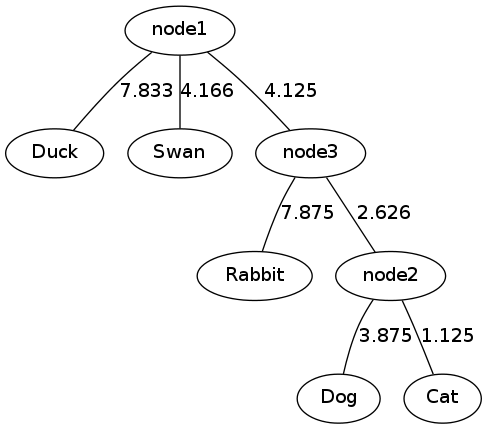
\includegraphics[scale=0.6]{./img/zadnji.png}
\caption{Konačno stablo}
\end{figure}

\chapter{Testiranje i usporedbe}
\section{Korišteni jezici}
Algoritam je implementiran u šest različitih jezika i to prema podjeli:
\begin{itemize}
	\item Filip Beć - \textbf{Objective-C}
	\item Zorana Ćurković - \textbf{Python}
	\item Goran Gašić - \textbf{Java}
	\item Melita Kokot - \textbf{Ruby}
	\item Dino Šantl - \textbf{C}
	\item Igor Smolkovič - \textbf{C++}
\end{itemize}

\section{Infrastruktura}
Algoritam kao ulaz uzima matricu udaljenosti. U praksi se algoritam \emph{Neighbor joining} koristi u kombinaciji s algoritmima poravnanja. Nakon što se genetski nizovi poravnaju računa se udaljenost između njih te je taj rezultat ulaz algoritma \emph{Neighbor joining}. Kako ne bi svaka implementacija algoritma u sebi sadržavala i algoritam poravnanja, napravljena je infrastruktura koja napravi poravnanja neovisno o implementaciji (jeziku). Infrastruktura tada određenoj implementaciji preda rezultate izvođenja poravnanja tj. udaljenosti između genetskih nizova. Osim pripreme ulaza, infrastruktura se brine za crtanje dobivenog grafa, jer je čisti tekstualni zapis grafa beskoristan za ljudsku interpretaciju. Infrastruktura se nalazi u mapi \emph{"Infra/"} u repozitoriju.

\subsection{Priprema ulaza - poravnanja}

Za pripremu ulaza koristi se skripta \emph{alignament.py} napisana u \emph{Python}-u. Koristi se biblioteka \emph{BioPython} gdje se nalazi programska podrška za \emph{Muscle}. \emph{Muscle} omogućava višestruko poravnanje genetskih nizova. Kao ulaz daje se datoteka u \emph{FASTA} formatu. Izlaz je skup genetskih nizova iste duljine.
 
Nakon koraka poravnanja potrebno je izračunati udaljenosti među dobivenim nizovima. Udaljenost se računa kao postotak poklapanja pripadajućih znakova u nizu gdje se zanemaruju procijepi. Na kraju se iz dobivenih postotaka računa udaljenost po Jukes-Cantorovom modelu.

Na temelju indeksa genetskog niza i udaljenosti između nizova stvara se ulaz u algoritam  \emph{Neighbor joining} tako da se u prvi red zapiše broj genetskih nizova, a nakon toga u $\frac{N(N-1)}{2}$ redova se zapisuju udaljenosti između nizova kao: "$i$ $j$ distance", gdje je uvijek $i<j$, a $i$ i $j$ su pripadajući identifikatori nizova.

\subsection{Crtanje grafa}

Kako bi se mogli vizualizirati rezultati algoritma generira se datoteka u \emph{DOT} jeziku koji služi za opisivje grafova. Tako napisan program (opis grafa) može se prevesti u neki od slikovnih formata (npr. png).

Implementacije algoritma \emph{Neighbor joining} kao izlaz daju skup bridova u obliku "$i$ $j$ distance", gdje su $i$ i $j$ čvorovi u stvorenom stablu, a \emph{distance} udaljenost između njih. Skripta \emph{generate\_graph.py} generira na temelju takvog izlaza (skupa bridova) opis grafa u \emph{DOT} jeziku.

\subsection{Pokretanje primjera}

Skripta napisana u \emph{bash} jeziku, \emph{nj\_process} spaja tri komponente infrastrukture - poravnanje nizova, implementaciju  \emph{Neighbor joining} algoritma i vizualizaciju dobivenog grafa. Skripta se koristi na sljedeći način: "\emph{./nj\_process program fasta\_datoteka}". 
Za određenu implementaciju u repozitoriju potrebno je pokrenuti npr.:\\ "\emph{./nj\_process ../Code/Santl/Bin/neighbour\_joining test1.fasta}".
Za druge implementacije dane su naredbe u \emph{README.md} u repozitoriju. Kao rezultat izvođenja infrastrukture dobija se sličan prikaz kao na slici \ref{ref:infra}.

\begin{figure}[htb]
\centering
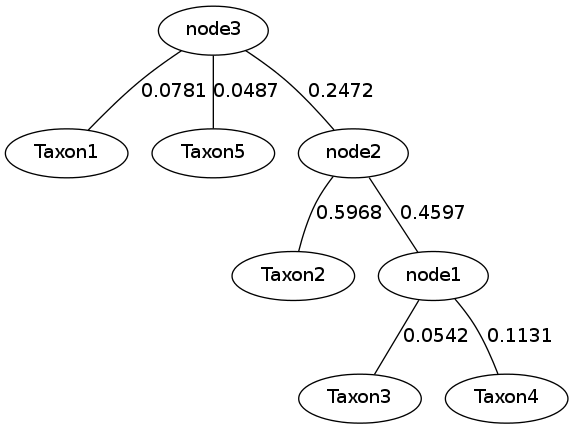
\includegraphics[scale=0.6]{./img/infra.png}
\caption{Primjer slike generirane pomoću infrastrukture}
\label{ref:infra}
\end{figure}

\newpage
\section{Testiranje}

Za testiranje implementacija napisane su skripte koje omogućavaju automatizirano ispitivanje i vizualizaciju rezultata. Ispitna struktura se nalazi u repozitoriju u mapi \emph{"Test/"}.

Testiranje obuhvaća tri cjeline: točnost, vrijeme izvođenja i korištena memorija. Komponentu točnosti nije se mogla utvrditi do kraja. Algoritam \emph{Neighbor joining} u svojoj definiciji ima nedeterminističko svojstvo. U algortmu nije definirano što se događa ako se u matrici \textbf{Q} pojave parovi čvorova koji imaju istu vrijednost. U tom slučaju može se uzeti bilo koji od njih i zato u ovisnosti o implementaciji izlazi algoritma mogu davati različita stabla. Zato su se kao testni primjeri uzele matrice udaljenosti koje daju jedinstvena stabla. Za to je korištena skripta u mapi \emph{"Test/"} pod nazivom \emph{check\_isomorphism.py} koja provjerava izomorfnost dvaju težinskih grafova.

Za ispitivanje vremena izvođenja i korištene memorije generirani su test primjeri različitih veličina (broja čvorova). Ispod se nalaze grafovi koji prikazuju mjerene veličine.

\subsection{Vrijeme izvođenja}

Vrijeme izvođenja algoritma testirano je nad brojem čvorova $N$=3, 5, 10, 50, 100, 150, 300, 500, 1000. Na slikama \ref{fig:time_100}, \ref{fig:time_50_300} i \ref{fig:time_150_1000} prikazane su različiti intervali i vremena izvođenja. Na intervalu $\left [ 150,1000 \right ]$ nisu prikazani skriptni jezici jer je fokus stavljen na druge jezike. 

\begin{figure}[!h]
\centering
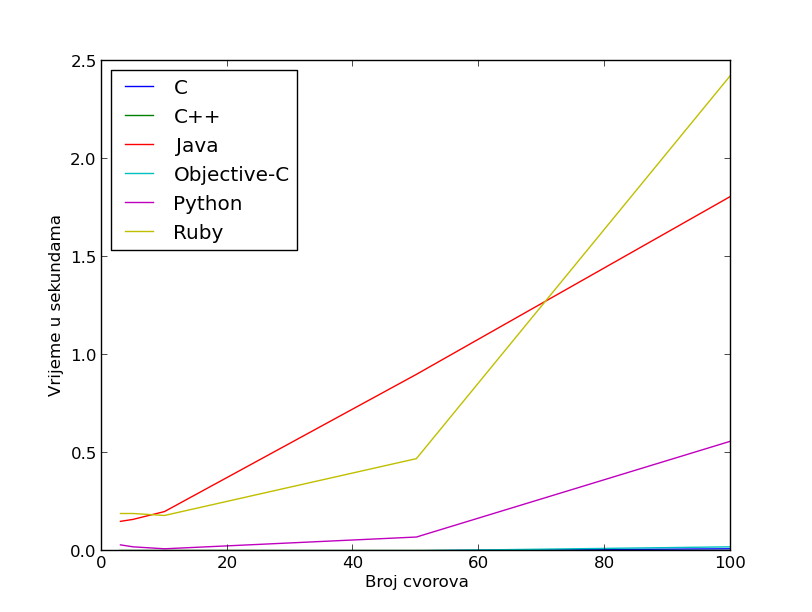
\includegraphics[scale=0.6]{./img/Primjeri_do_100.png}
\caption{Vremena izvođenja algoritama za veličine od 3 do 100 čvorova}
\label{fig:time_100}
\end{figure}

\begin{figure}[!h]
\centering
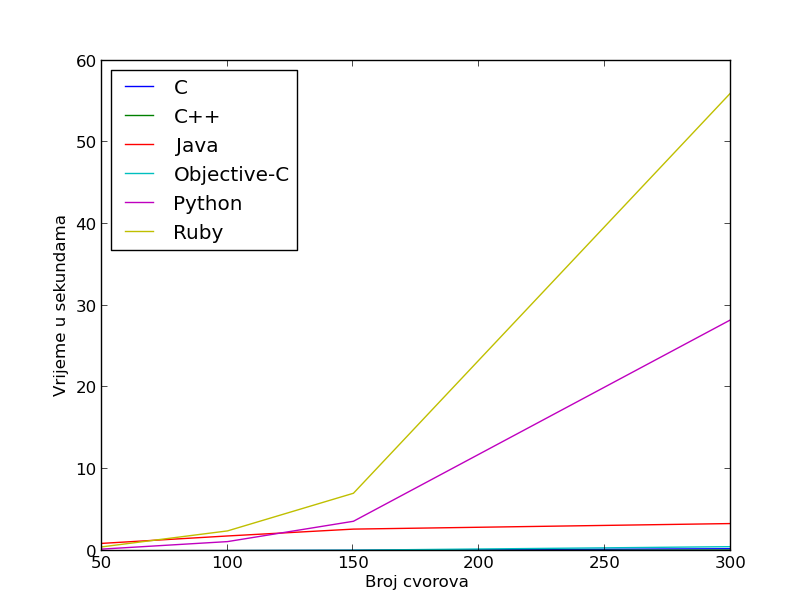
\includegraphics[scale=0.6]{./img/Primjeri_50_300.png}
\caption{Vremena izvođenja algoritama za veličine od 50 to 300 čvorova}
\label{fig:time_50_300}
\end{figure}

\begin{figure}[!h]
\centering
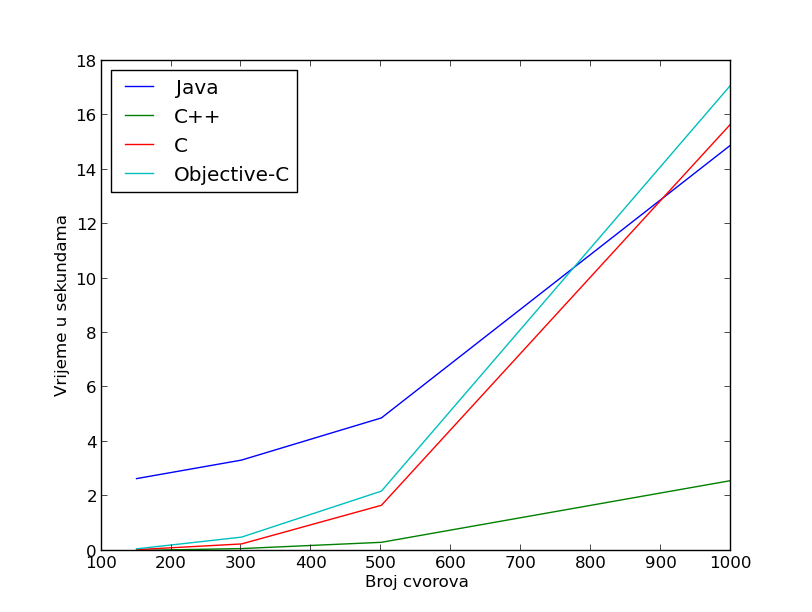
\includegraphics[scale=0.6]{./img/Primjeri_150_1000.png}
\caption{Vremena izvođenja za primjere od 150 do 1000 čvorova}
\label{fig:time_150_1000}
\end{figure}

\newpage

\subsection{Korištena memorija}

Mjerena je maksimalna količina memorije u nekom trentku za vrijeme izvođenja procesa. Jednako kao i za vrijeme, implementacije su ispitane nad brojem čvorova $N$=3, 5, 10, 50, 100, 150, 300, 500, 1000. U nastavku se nalaze različiti grafovi koji prikazuju različite intervala za broj čvorova. 

\begin{figure}[!h]
\centering
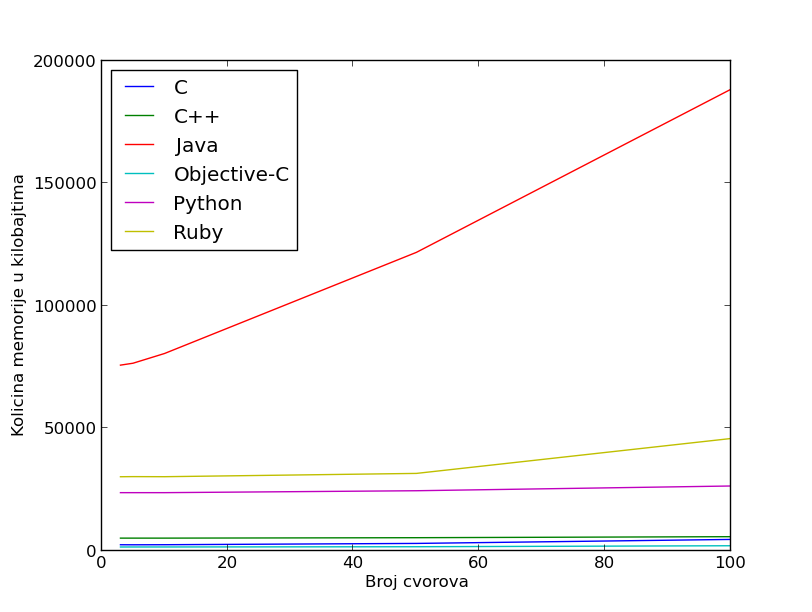
\includegraphics[scale=0.6]{./img/memorija_100.png}
\caption{Korištena memorija u kilobajtima do 100 čvorova}
\label{fig:memorija_100}
\end{figure}

\begin{figure}[!h]
\centering
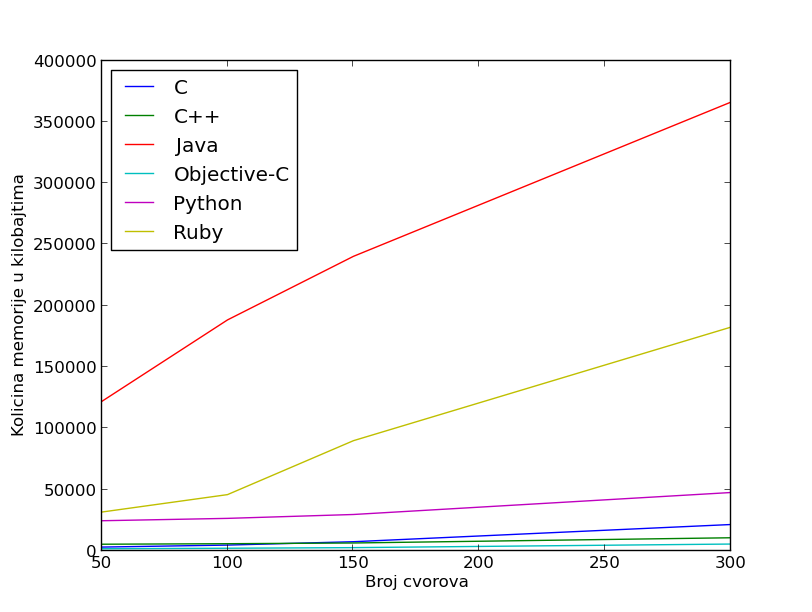
\includegraphics[scale=0.6]{./img/memorija_300.png}
\caption{Korištena memorija u kilobajtima od 50 do 300 čvorova}
\label{fig:memorija_300}
\end{figure}

\begin{figure}[!h]
\centering
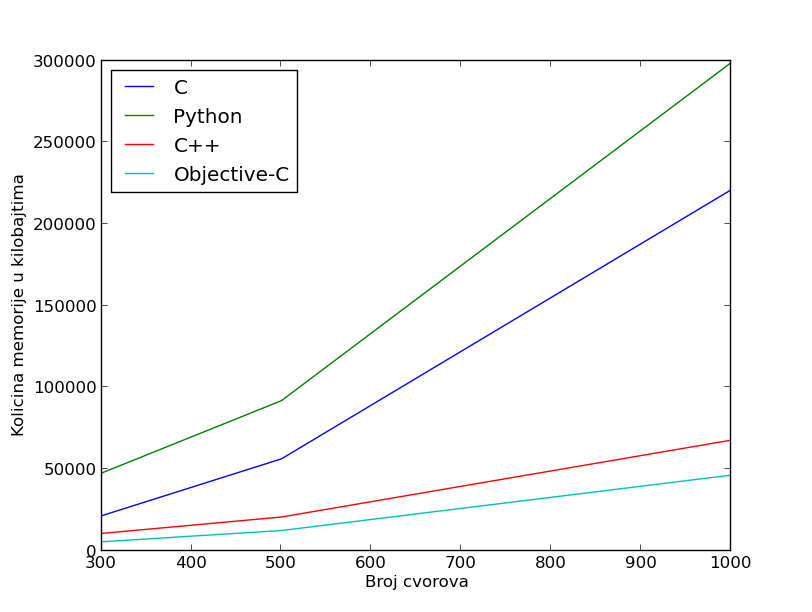
\includegraphics[scale=0.6]{./img/memorija_1000.png}
\caption{Korištena memorija od 300 do 1000 čvorova}
\label{fig:memorija_1000}
\end{figure}

\section{Rezultati}
Algoritam se može implementirati u apriornoj vremenskoj složenosti $O(N^3)$, gdje je $N$ broj čvorova. Mjerenja su pokazala da implementacija algoritma ovisi o jeziku u kojem je algoritam ostvaren. Tako generalno možemo reći da niži programski jezici daju bolje rezultate, dok skriptni jezici očekivano daju nešto lošja vremena izvođenja.

Graf vremena izvođenja do sto čvorova (slika \ref{fig:time_100}) pokazuju da viši programski jezik \emph{Java} i skriptni jezici \emph{Ruby} i \emph{Python} imaju puno veća vremena izvođenja od ostalih jezika, što je i očekivano. Zanimljiv je graf na slici \ref{fig:time_50_300} gdje se vidi da za malo veći broj čvorova programski jezik \emph{Java} ima puno manje vrijeme izvođenja od skiptnih jezika. Za nešto veći broj čvorova, do njih 1000 (slika \ref{fig:time_150_1000}), pokazuje se da se \emph{Java} može mjeriti s ostalim jezicima. Najbolje vrijeme izvođenja imala je implementacija u \emph{C++} programskom jeziku, što je i očekivano jer je \emph{C++} dovoljno nizak jezik, a opet koristi bibliotetke struktura koje su optimizirane. Jezici \emph{Objective-C} i \emph{C} pokazuju gotovo identične rezultate.

Rezultati ispitivanja korištene memorije jednako tako su očekivani. \emph{Java} programski jezik troši najviše memorije zbog popratnih troškova virtualnog stroja. Skriptni jezici troše nešto više memorije ali ne znatno od ostalih jezika. Implementacija u jeziku \emph{C} troši nešto više memorije zbog toga jer je napravljen \emph{trade-off} između čitkosti koda i efikasnosti. Jezici \emph{C++} i \emph{Objective-C} daju najbolje rezultate jer su korištene efikasne strukture odnosno \emph{Objective-C} prilagođen je za mobilne uređaje koji ne bi trebali trošiti puno memorije.

\chapter{Zaključak}

Ishod projekta pokazao je kako određeni programski jezici utjeću na implementaciju algoritama, konkretno na algoritam koji se koristi u bioinformatici. Pokazalo se da niski programski jezici poput \emph{C} jezika mogu dati dobre rezultate, ali implementacija algoritma je kompleksnija. \emph{C++} jezik dobar je izbor. Iako na nižoj razini, omogućuje da se uz znatno manji broj linija i uz korištenje ugrađenih struktura podataka ostvare vrlo dobri rezultati. \emph{Java} je također dobar izbor jer se pokazalo da vrijeme izvođenja na većim test primjerima nije lošije od ostalih jezika, a dovoljno je na visokom nivou da se primjerice izbjegava ručno upravljanje memorijom. Skriptni jezici nisu dobar izbor za krajnji produkt, ali dobar su izbor za implementaciju prototipa algoritma. Razvoj algoritma u skriptnim jezicima je brz što omogućava efikasno eksperimentiranje s različitim parametrima. \emph{Objective-C} je poseban slučaj. Pokazalo se da se može koristiti u implementaciji algoritama, samo što nije namijenjen znanstvenicima koji se primarno bave biologijom.

\bibliography{literatura}
%\bibliographystyle{fer} %promijena za citiranje po redu ieeetr
\bibliographystyle{ieeetr}

\begin{comment}
\begin{sazetak}
Simbolička regresija je postupak otkrivanja matematičkog izraza u skupu podataka. Daje se pregled metoda za simboličku regresiju s naglaskom na genetsko programiranje. Obrađuju se problemi kao što su domene funkcija (nisu definirane na cijelom skupu realnih brojeva). Problemi se rješavaju intervalnom aritmetikom i linearnim skaliranjem. Na kraju se ukratko opisuje mogućnost paralelizacije i primjene. 

\kljucnerijeci{genetsko programiranje, s}

\end{sazetak}

% TODO: Navedite naslov na engleskom jeziku.
\engtitle{Application of graphics coprocessors for program execution on stream programming model}

\begin{abstract}


\keywords{GPU, StreamIt, Sponge, StreamGate, CUDA, stream model, filter, optimization, graphics card}
\end{abstract}
\end{comment}

\end{document}
